\chapter{Přírodou inspirované počítání}
\section{Genetické algoritmy, genetické a evoluční programování.}
\subsection{Evoluční algoritmy}
\label{ea}
\textbf{Evoluční algoritmy (EA)} je souhrnné označení pro všechny výpočetní metody inspirované evolucí. Historicky se nejdříve paralelně vyvíjely 3 metodiky: genetické algoritmy, evoluční strategie a evoluční programování. Až později došlo k jejich seskupení pod společný zastřešující název: evoluční algoritmy (někdy také evoluční počítání).

EA jsou populační stochastické prohledávací algoritmy. Obecně se hodí spíše označení meta-algoritmus, jelikož pro specifické problémy se vytváří doménově specifické varianty EA s doménově danou reprezentací a vlastními implementacemi evolučních operátorů. Obecně platí \uv{no free lunch theorem} -- tj. neexistuje jeden ultimátní nejlepší algoritmus pro všechny typy problémů.

Základní struktura obecného EA je následující:
\begin{enumerate}
	
	
	\item vytvoř náhodnou iniciální populaci $P(t=0)$, ohodnoť $P(0)$
	\item dokud není splněna ukončovací podmínka:
	\begin{enumerate}
		
		
		\item rodičovská selekce podle fitness
		\item křížení s pravděpodobností $p_c$
		\item mutace s pravděpodobností $p_m$
		\item ohodnocení nové populace, environmentální selekce do $P(t+1)$
	\end{enumerate}
\end{enumerate}
\begin{figure}[H]
	\centering
	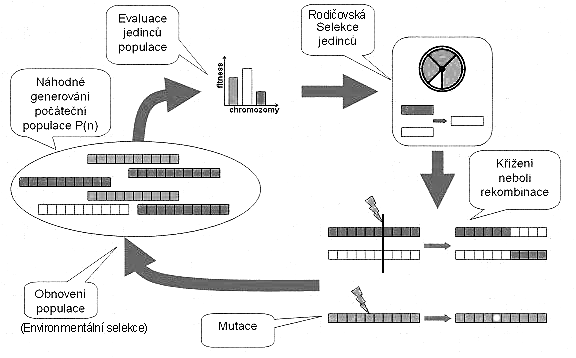
\includegraphics[width=0.8\textwidth]{img/ea.png}
\end{figure}

\subsection{Genetické algoritmy (GA)}
Původní Hollandův GA (dnes označován jako Simple GA, SGA) je nejstarší a nejjednodušší varianta EA, jejímž klíčovým rysem je to, že jedinci jsou \textbf{binární řetězce}. Používá ruletovou selekci (rodičovskou, environmentální se nepoužívá), 1-bodové křížení, bitové mutace (viz níže). V původním Hollandově návrhu je i operátor \textit{inverze}, který obrátí část řetězce, ovšem se zachováním významu bitů. Inverze se ukázala být nevýhodnou.


%TODO GA

\subsection{Genetické programování (GP)}
\begin{wrapfigure}{r}{0.3\textwidth}
\centering
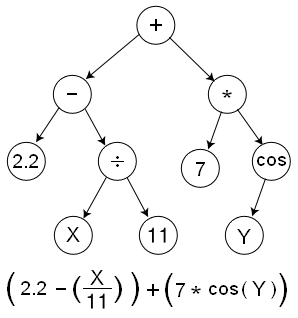
\includegraphics[width=0.25\textwidth]{img/gp.png}
\end{wrapfigure}
Tento pojem označuje genetické algoritmy, v nichž je jedincem v populaci počítačový \textbf{program}. Myšlenkou tedy je, že budeme evolvovat počítačový kód, který za nás bude řešit problémy. Duchovním otcem GP je John Koza. V jeho původní práci jsou programy reprezentovány jako syntaktické stromy, kde listy jsou proměnné a konstanty, vnitřní uzly jsou operace. \textbf{Křížení} je výměna podstromu, \textbf{mutací} se používá několik typů: mutace konstant, výměna uzlu stejné arity, permutace podstromů, záměna neterminálu za terminál apod. \textbf{Fitness} je poměrně jednoduchá: spustit vygenerovaný program na testovacích datech a ohodnotit, nakolik řeší daný problém.

Vylepšení základního principu je použití \textbf{automaticky definovaných funkcí (ADF)}. To jsou samostatné stromy, které mají omezenou množinu terminálů i neterminálů a jsou charakterizovány svou aritou. Volání nějaké ADF je pak novým terminálem, který se může vyskytnout v listech. Celý program pak sestává z hlavního stromu a několika vedlejších stromů ADF. Genetické operace GP pracují buď jen v rámci hlavního programu nebo v rámci ADF.

GP se často potýká s problémem bobtnání (\textbf{bloat}), tj. programy mají tendenci narůstat. V praxi se to řeší restrikcí velikosti či hloubky stromu, a to buď jako penalizující člen ve fitness a nebo jako kontrola (a případná eliminace) nově vznikajících jedinců. Zavádí se taky \textit{anti-bloat} operátory, tedy křížení a mutace, které jedince nezvětšují, případně jej rovnou zmenšují.

Kromě stromů lze použít i jiné struktury. \uv{Cestou dolů} jsou \textbf{lineární GP}, tj. program je lineární sekvence příkazů. To vede k jednodušším operátorům i celkové reprezentaci, rovněž rychlejší emulaci běhu; nicméně je tu velké riziko toho, že vznikne nesmyslný program. \uv{Cestou nahoru} jsou \textbf{grafové GP}, kde program je (často acyklický) graf. Vznikly nejprve jako rozšíření na paralelní programy, později získaly obecnější tvar a dnes se používají např. pro evoluci obvodů či neuronových sítí. Kvůli větší komplexitě reprezentace jsou komplikovanější i genetické operátory.

\subsection{Evoluční programování (EP)}
Evoluční programování je jeden z nejstarších směrů vývoje evolučních algoritmů, dokonce ještě o něco starší než Hollandovy GA (60. léta). Průkopníkem je Lawrence Fogel. Zásadní myšlenkou je vyvinout \uv{umělou inteligence}, konkrétně agenta, který bude umět předpovídat stav prostředí -- jinými slovy bude umět odvodit patřičnou akci v reakci na prostředí, v němž se nachází. Agent je zde reprezentován \textbf{konečným automatem}, prostředí je pak \textbf{sekvence symbolů konečné abecedy}.

Samotná evoluce pak vypadá takto: jedinci v populaci jsou konečné automaty, těm jsou předkládány vstupy. Jejich výstup je vždy porovnán s následujícím vstupem v posloupnosti. Fitness je úspěšnost predikce, přičemž se může měřit různě: vše nebo nic, absolutní chyba, mean square error. Často je do fitness započítána i velikost automatu.

\textit{Každý} automat podstoupí mutaci, která může mít různou \uv{intenzitu} -- od malých, \uv{kosmetických} změn po radikální. Příklady mutací jsou: změna výstupního symbolu, změna následného stavu, přidání stavu, odebrání stavu, změna počátečního stavu, \dots Noví jedinci jsou ohodnoceni a poté je vybráno (z nových i starých najednou) $N$ jedinců do nové populace. Výběr probíhá buď turnajem, nebo deterministicky (tj. vezme se $N$ nejlepších jedinců. (Pozn.: V původním algoritmu není nijak omezeno, kolik potomků může být vygenerováno z jednoho rodiče, ani že velikost populace musí zůstávat konstantní.)

\textbf{Křížení neexistuje (!)}. 

V dnešní době se EP vyvinulo do obecnější podoby. Zakódování jedinců je velmi benevolentní a mělo by být přirozené pro daný problém (často genotyp = fenotyp). Používá se více \uv{chytrých mutací}, které jsou těsně přizpůsobeny problému a dané reprezentaci. Křížení se typicky nepoužívá. Rodičovská selekce je prostá: každý jedinec se vybere právě jednou. Environmentální selekce je turnajová na spojené populaci rodičů a potomků.

Jelikož se EP vyvíjelo paralelně s GA i ES, jsou mezi nimi nevyhnutelně mnohé podobnosti. Pojďme si tyto metody porovnat.

\subsubsection{EP vs. GA}
V GA jsou jedinci sekvence symbolů abecedy, původně pouze binární, dnes už vcelku libovolné. V EP není žádné omezení na podobu reprezentace a typicky je přizpůsobena problému (jedinec může být např. neuronová síť). 

Mutace funguje rovněž trochu jinak. V EP máme škálu mutací od malých změn až po radikální zásahy, přičemž pravděpodobnost aplikace mutace je nepřímo úměrná její závažnosti. Celková závažnost mutací se rovněž může snižovat v průběhu konvergence k optimálnímu řešení.

Zjevným rozdílem je rovněž absence křížení u EP.

\subsubsection{EP vs. ES}
Pokud je jedincem v EP posloupnost reálných čísel, začínají být velice podobné evolučním strategiím. EP dokonce také mohou být \textit{self-adaptive}, tj. jedinec nese kromě genotypu i parametry ovlivňující evoluci, konkrétně míru závažnosti mutací (rozptyl gaussovské mutace).

Existují však rozdíly: EP používá turnajovou selekci, ES deterministicky odstraňuje dané množství nejhorších řešení. Druhým rozdílem je absence křížení u EP, zatímco ES je často implementuje. 

\subsubsection{Význam křížení}
Malá odbočka: trpí EP tím, že nemá křížení? Pomáhá vlastně křížení, nebo stačí mutace? Jones (1995) provedl tzv. \uv{headless chicken epxeriment}: porovnával klasické GA a GA, kde je klasické křížení nahrazeno \uv{náhodným křížením}. To funguje tak, že se dva vybraní jedinci nezkříží mezi sebou, namísto toho se pro každého z nich vygeneruje partner jako náhodná sekvence z domény (tj. například náhodný binární vektor správné délky). Pak se provede jednobodové křížení a od každého rodiče se vybere jeden potomek. Jones označil tento operátor jako \textit{headless chicken} -- stejně jako bezhlavé kuře pobíhající po dvorku není doopravdy kuře (protože mu něco důležitého chybí), tak ani toto \uv{náhodné křížení} není vlastně křížení, protože při něm vůbec nedochází ke kontaktu mezi jedinci. Jedná se ve skutečnosti o jakousi makromutaci.

Pointou experimentu bylo porovnat výkonnost obou variant a určit, nakolik opravdové křížení skutečně pomáhá. Závěrem bylo konstatování, že pokud má problém jasně definované stavební bloky, pak křížení skutečně pomáhá (především na začátku evoluce), zatímco pokud nejsou bloky zřejmé, pak křížení příliš nepomáhá (výkon obou variant byl srovnatelný).

\section{Teorie schémat, pravděpodobnostní modely jednoduchého genetického algoritmu.}
\subsection{Schémata}
\textbf{Schéma} v kontextu genetických algoritmů (tj. jedinec je slovo v abecedě \{0,1\}) je reprezentace množiny jedinců jako slova v abecedě \{0,1,*\}, kde * označuje libovolný symbol (\uv{žolík}). Například schéma 0*11* reprezentuje množinu jedinců \{00110, 00111, 01110, 01111\}. Platí následující:
\begin{itemize}
	
	
	\item schéma s $r$ * reprezentuje $2^r$ jedinců
	\item jedinec délky $m$ je reprezentován $2^m$ schématy
	\item je $3^m$ schémat délky $m$
	\item v populaci velikosti $n$ je $2^m$ až $n\cdot2^m$ schémat
\end{itemize}
Pro schéma S lze definovat následující vlastnosti:
\begin{description}
	
	
	\item[Řád schématu o(S):] počet pevných pozic (0 a 1) 
	\item[Definující délka d(S):] vzdálenost mezi první a poslední pevnou pozicí
	\item[Fitness F(S)] průměrná fitness odpovídajících jedinců v populaci
\end{description}

\noindent\textbf{Věta o schématech (VoS):} \textit{Krátká schémata s nadprůměrnou fitness a malým řádem se v populaci během GA exponenciálně množí.}


\begin{proof} Budeme zkoumat, co se děje s konkrétním schématem $S$ během selekce, křížení a mutace.

Nechť $P(t)$ je populace v čase $t$, $n$ je velikost populace, $m$ je délka jedinců v populaci, $C(S,t)$ je četnost schématu $S$ v populaci $P(t)$ (tj. počet jedinců v $P(t)$ reprezentovaných $S$). Budeme odhadovat $P(S, t+1)$.

\textit{Selekce:} Schéma $S$ má pravděpodobnost vybrání
$$p_s(S) = \frac{F(S)}{\sum\limits_{u \in P(t)}F(u)}$$
Tedy 
$$C(S,t+1) = C(S,t) \cdot n \cdot p_s(S)$$
neboť provádím $n$ výběrů do nové populace pomocí ruletové selekce, přičemž na ruletě zabírají jedinci odpovídající schématu $S$ právě $C(S,t) \cdot p_s(S)$ procent místa. Ekvivalentně lze psát
$$C(S,t+1) = C(S,t) \cdot \frac{F(S)}{\frac{\sum_{u \in P(t)}F(u)}{n}} = C(S,t) \cdot \frac{F(S)}{F_{avg}(t)}$$
kde $F_avg(t)$ označuje průměrnou fitness v populaci $P(t)$. 

Představme si, že schéma $S$ je nadprůměrné o $\varepsilon$\,\%, tj. $F(S) = F_{avg}(t) + \varepsilon\cdot F_{avg}(t)$. Pak 
$$C(S,t+1) = C(S,t)(1+\varepsilon)$$
$$C(S,t+1) = C(S,0)(1+\varepsilon)^t$$
Tedy četnost nadprůměrných schémat roste geometrickou řadou.

\textit{Křížení:} Předpokládáme klasické jednobodové křížení. Pravděpodobnost, že schéma $S$ křížení nepřežije, je 
$$p_{death}(S) = \frac{d(S)}{m-1}$$
a tedy pravděpodobnost přežití je 
$$p_{surv}(S) \geq 1 - p_c \cdot \frac{d(S)}{m-1}$$
kde $p_c$ je pravděpodobnost křížení. Všimněte si nerovnosti: je totiž šance, že i když se bod křížení \uv{trefí} dovnitř schématu, tak část doplněná s druhého rodiče bude pořád odpovídat schématu a celkově tedy schéma přežije. Zjevné je to například při křížení dvou totožných jedinců (tam schéma přežije vždy).

\textit{Mutace:} Pravděpodobnost změny jednoho bitu je $p_m$, pravděpodobnost přežití schématu je tedy 
$$p_{surv}(S) = (1-p_m)^{o(S)}$$
$$p_{surv}(S) \approx 1 - p_m \cdot o(S)$$
Poslední aproximace funguje pro $p_m \ll 1$.

Dohromady tedy dostáváme:
$$C(S,t+1) \geq C(S,t) \cdot \frac{F(S)}{F_{avg}(t)} \cdot \left(1 - p_c \cdot \frac{d(S)}{m-1} - p_m \cdot o(S)\right)$$
\end{proof}

\textbf{Hypotéza o stavebních blocích (HoSB)} GA hledá suboptimální řešení problému rekombinací krátkých, nadprůměrných s malým řádem schémat (\uv{building blocks}).

\subsubsection{Důsledky VoS}
GA pracuje s $n$ jedinci, ale implicitně vyvíjí mnohem více schémat: $2^m$ až $n\,2^m$ (implicitní paralelismus). Holland tvrdí, že za splnění jistých předpokladů ($n = 2^m$, schémata zůstávají nadprůměrná, \dots) platí, že počet schémat, kterým se v GA dostává exponenciálního růstu je úměrný $n^3$. 

GA také optimálně řeší problém explorace a exploatace, což lze ukázat na analogii s tzv. \textbf{2-rukým banditou}: \textit{Mám N mincí, ruce bandity (= hrací automat) vyplácí se střední hodnotou $m_1$ resp. $m_2$ a rozptylem $s_1$ resp. $s_2$, cílem je maximalizovat zisk. Analytickým řešením je alokovat exponenciálně více pokusů pro právě vyhrávající ruku.} GA rovněž alokuje exponenciálně mnoho nadějným schématům. Nejdříve se myslelo, že GA hraje $3^m$-rukého banditu, tj. všechna schémata jsou konkurenční ruce. Ve skutečnosti se hraje více her, v nichž schémata soutěží o konfliktní pevné pozice: schémata řádu $k$ soutěží právě o těch $k$ pozic -- hrají spolu $2^k$-rukého banditu. To stále není úplně přesné, protože na rozdíl od bandity, kde jsou ruce nezávislé, nesampluje GA schémata nezávisle.

Problémem také je, že GA často neodhadne správně skutečnou fitness schémat. Např. je-li F(111*\dots*)~= 2, F(0*\dots*) = 1 a jinak F(x) = 0, pak platí F(1*\dots*) = $\frac{1}{2}$, F(0*\dots*) = 1. Jenže GA odhadne F(1*\dots*) $\approx$ 2, protože 111*\dots* v populaci převáží. Tomuto se říká \textit{kolaterální konverence}, tj. jakmile se někam začne konvergovat, už nejsou schémata samplována rovnoměrně a fitness se neodhadne správně. Podobným problémem je velký rozptyl fitness (např. 1*\dots* z předchozího příkladu). GA bude nejspíše konvergovat tam, kde je fitness větší $\rightarrow$ chybný odhad statické fitness.


\subsection{Pravděpodobnostní modely}
Od 90. let se objevují snahy přesně modelovat chování GA, konkrétně: jak přesně vypadají populace, zobrazení přechodu k další populaci, vlastnosti tohoto zobrazení, asymptotické chování jednoduchého GA. Existují modely pro konečné i nekonečné populace.

\subsubsection{Ještě jednodušší jednoduchý GA (JJJGA)}
Pro jednodušší tvorbu modelů byl původní jednoduchý GA ještě o něco zjednodušen a formalizován takto:
\begin{itemize}
	
	
	\item inicializuj náhodnou počáteční populaci binárních řetězců $x$ délky $l$
	\item dokud nenajdeš dost dobré $x$:
	\begin{itemize}
		
		
		\item dokud nenaplníš novou populaci:
		\begin{itemize}
			
			
			\item vyber selekcí 2 jedince, zkřiž je s pravděpodobností $p_c$, jednoho potomka zahoď
			\item mutuj každý bit nového řetězce s pravděpodobností $p_m$
			\item vlož do nové populace
		\end{itemize}
	\end{itemize}
\end{itemize}

\subsubsection{Analýza}
Každý jedinec je tedy binární řetězec délky $l$, což lze chápat jako binární zápis nějakého čísla [0, \dots, $2^l-1$] (např. 00000111 je 7). Populace v čase $t$ je reprezentována dvěma vektory $p(t)$ a $s(t)$, oba délky $2^l$. Číslo $p_i(t)$ vyjadřuje, kolik procent populace zabírá řetězec $i$; číslo $s_i(t)$ vyjadřuje pravděpodobnost selekce řetězce $i$.

Dále definujeme matici $F$ takto: $F(i,i) = f(i); F(i,j) = 0$ pro $i \neq j$. Hodnota $f(i)$ je fitness jedince $i$. Pak můžeme definovat vztah vektorů $s(t)$ a $p(t)$ jako
$$s(t) = \frac{F \cdot p(t)}{\sum\limits_{j=0}^{2^l-1} F(j,j) \cdot p_j(t)}$$

Naším ideálem je definovat matici G, která realizuje jeden krok JJGA, tj. $p(t+1) = G \cdot p(t)$, nebo obdobně $s(t+1) = G \cdot s(t)$. Toto zobrazení bude fungovat jako složení dvou dílčích zobrazení: matice F (fitness) a matice M (mutace a křížení). 

Nejprve uvažme $G=F$ (tj. nemáme žádné genetické operátory). Platí $E(p(t+1)) = s(t)$, kde $E$ je střední hodnota. Pak díky $s(t+1) \sim F \cdot p(t+1)$ (liší se jen o multiplikativní odchylku) můžeme psát $E(s(t+1)) \sim F \cdot s(t)$. V případě konečné populace nám výběrové chyby mohou způsobit odchylku od $E()$, obecně čím větší populace, tím menší odchylka. U nekonečné populace by to bylo přesné.

Nyní se podívejme na situaci $G = M$, tedy neřešíme selekci. Zde využijeme pomocnou veličinu $r(i,j,k)$, která udává pravděpodobnost, že z $i$ a $j$ vznikne $k$. Když tuto veličinu známe, pak lze vyjádřit 
$$E(p_k(t+1)) = \sum\limits_{i=0}^{2^l-1} \sum\limits_{j=0}^{2^l-1} s_i(t) \cdot s_j(t) \cdot r(i,j,k)$$
Funkci $r(i,j,k)$ lze analyticky spočíst.\footnote{\url{http://ktiml.mff.cuni.cz/~neruda/eva2-13.pdf}}

Závěr: JJGA pracující prostřednictvím $G$ je dynamický systém, $p(t)$ či $s(t)$ jsou body (trajektorie). Neznáme jeho pevné body, můžeme však vyjádřit pevné body jednotlivých zobrazení: Pevné body F jsou populace se stejnou fitness, stabilní pevný bod F je maximální stejná fitness. (Jediný) pevný bod M: stejné pravděpodobnosti $s$ (resp. stejné zastoupení jedinců $p$). Kombinace míchání M a ostření F odpovídá fenoménu \textit{punctuated equilibria} (známe z biologie).

\subsubsection{Konečné populace}
Pro konečné populace lze definovat GA jako \textit{markovovský řetězec}, tj. stochastický proces v systému se stavy a přechody mezi stavy s definovanými pravděpodobnostmi. Pravděpodobnost přechodu závisí vždy pouze na předchozím stavu. Jeden stav systému je jedna konkrétní populace. Populací o $n$ jedincích délky $l$ je $N = \binom{n+2^l-1}{2^l-1}$, matice pravděpodobností přechodů je $N\times N$, podrobnější rozbor opět v Nerudových slajdech.

Dokázala se korespondence ideálního JJGA s nekonečnou populací a modelu s konečnou populací (pro $n \rightarrow \infty$).






\section{Evoluční strategie, diferenciální evoluce, koevoluce, otevřená evoluce.} 
\subsection{Evoluční strategie}
\textbf{Evoluční strategie (ES)} je metoda pro optimalizaci reálných funkcí, která je výjimečná tím, že jako první používala \textit{self-adaptation}, tj. parametry evoluce byly součástí jedince -- šlo tedy o \uv{evoluci evoluce}. Evolvovaný jedinec se tedy skládá z \textbf{genetických parametrů} ovlivňujících chování a \textbf{strategických parametrů} ovlivňující evoluci.

Vznikly v 60. letech, autoři \textbf{Rechenberg a Schwefel.} ES jsou jedna z větví evolučních algoritmů (anglicky se jako \uv{umbrella term} používá buď \textit{Evolutionary Algorithms} nebo \textit{Evolutionary Computation}), nicméně nevyčlenily se v průběhu, jak by se dalo čekat. ES se vyvíjely paralelně s GA a EP (evolučním programováním), až později došlo k seskupení těchto tří metod pod jeden společný obor.

\subsubsection{Notace}
\begin{description}
	
	
	\item[\textit{M}] počet jedinců v populaci
	\item[\textit{L}] počet vznikajících potomků
	\item[\textit{R}] počet rodičů každého nového jedince
\end{description}
Doporučení: $M > 1$, $L > M$ aby se vytvořily různé selekce (např. $L \approx 7 \cdot M$)

\subsubsection{Varianty}
\begin{description}
	
	
	\item[\textit{(M+L)} ES] -- M jedinců do nové populace je vybráno z M+L starých i nových jedinců
	\item[\textit{(M,L)} ES] -- M nových jedinců je vybráno jen z L nových potomků (tato varianta se ukázala být robustnější vůči uvíznutí v lokálních extrémech)
\end{description}

\subsubsection{Kódování, genetické operátory}
Jedinec je tvaru $C(i) = [G_n(i), S_k(i)], k \in \{1, n, 2n\}$, tedy první část je samotný genotyp, druhá část jsou parametry evoluce, konkrétně \textbf{hodnoty standardních odchylek floating point mutací}. Podle hodnoty $k$ rozlišujeme 3 varianty:
\begin{description}
	
	
	\item[k=1]: jedna společná odchylka pro všechny parametry
	\item[k=n]: nekorelované mutace; geometricky se mutuje po elipse rovnoběžné s osami
	\item[k=2n]: korelované mutace, odpovídají mutování z n-rozměrného normálního rozdělení. 
	Pro uložení korelační matice stačí n-rozměrný vektor (???). Tato matice odpovídá matici rotace (tj. elipsa se natočí v optimálním směru).
\end{description}

\begin{figure}[h]
	\centering
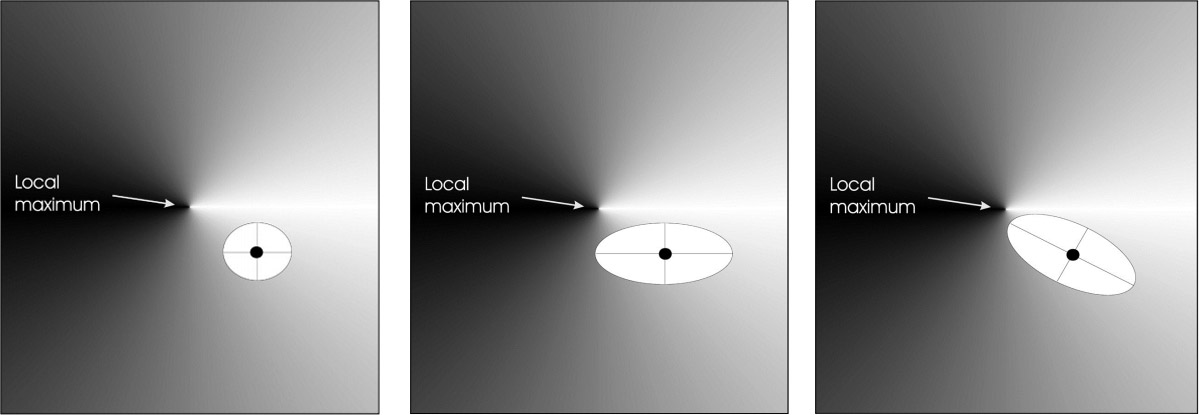
\includegraphics[width=0.7\textwidth]{img/ES_varianty_k.jpg}
\end{figure}

\textbf{Populační cyklus} vypadá takto:
\medskip

\begin{minipage}{\linewidth}
	\begin{lstlisting}[frame=single]
n=0, randomly init population P[n] of size M
evaluate fitness of individuals in P[n]
while not good enough:
	repeat L times:
		choose R parents
		crossover, mutate, evaluate new individual
	choose M new individuals (by the type of ES)
	n++
	\end{lstlisting}
\end{minipage}

Nový jedinec je akceptován pouze tehdy, je-li lepší než rodič -- pak rodiče nahradí.

\textbf{Mutace} jedince probíhá takto: \textit{genetické} parametry (genotyp) jsou změněny přičtením náhodného čísla s norm. rozdělení s příslušnou odchylkou (a případně i rotací). \textit{Strategické} parametry = odchylky jsou zvětšeny nebo zmenšeny podle \uv{pravidla $1/5$}, což heuristika, která říká, že nejlepší je, když má mutace úspěšnost 20\,\% (tzn. při menší zvyš odchylku, při větší sniž). V případě varianty s rotacemi jsou mezi strategickými parametry také hodnoty rotací -- ty se mutují jednoduše přičtením náhodného čísla z N(0,1).

\textbf{Křížení} je uniformní, typicky více rodičů. Podle velikosti R mluvíme o lokálním (R=2) nebo globálním (R=M). Může být diskrétní (použij hodnotu náhodně vybraného rodiče) nebo aritmetické (průměr).

\subsubsection{CMA-ES}
Dnes nejkomplexnější verzí je \textbf{CMA-ES} (Correlation Matrix Adaptation ES). Udržuje se korelační matice proměnných, která se inkrementálně aktualizuje po každém kroku metodou maximum-likelihood.

\subsection{Diferenciální evoluce}
Alternativní algoritmus spojité optimalizace, který funguje dobře i pro funkce které jsou nediferencovatelné, nespojité, zašuměné, neseparabilní nebo vysoce podmíněné. Každý jedinec prochází opakovaně cyklem \textbf{mutace} $\rightarrow$ \textbf{křížení} $\rightarrow$ \textbf{selekce}. Během mutace dochází k posunu \uv{podle ostatních}, tj. jedinec se posouvá ve směru populace. DE je také invariantní vůči rotaci či škálování prohledávaného prostoru.
\begin{figure}[H]
	\centering
	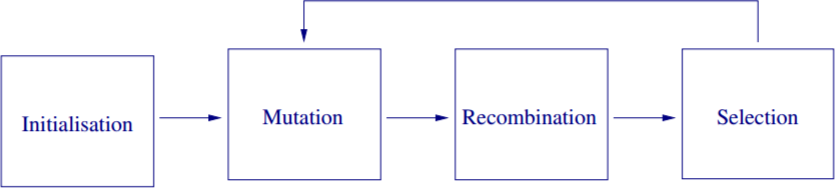
\includegraphics[width=0.7\textwidth]{img/de_scheme.png}
\end{figure}

\subsubsection{Mutace}
V populaci $p$ zvolíme pro jedince $x_{i,p}$ tři různé jedince: $x_{a,p}$, $x_{b,p}$ a $x_{c,p}$. Definujeme donora: $$v_{i,p+1} = x_{a,p} + F \cdot (x_{b,p} - x_{c,p})$$ kde $F \in \langle 0; 2 \rangle$ je parametr mutace.
\subsubsection{Křížení}
Uniformní křížení původního jedince s donorem. Parametr $C$ určuje pravděpodobnost změny, $rand_{ij} \in \langle0,1\rangle$ je pseudonáhodné číslo. Číslo $I_{rand}$ je náhodný index z $\langle 1,2,...D\rangle$, kde $D$ je délka jedince. Pak vytvoříme pokusný vektor $u_{i,p+1}$ jako:
$$u_{i,p+1}[j] = v_{i,p+1}[j] \leftrightarrow rand_{ji} \leq C \lor j = I_{rand}$$
$$u_{i,p+1}[j] = x_{i,p}[j] \leftrightarrow rand_{ji} > C \land j \neq I_{rand}$$

Díky $I_{rand}$ je zajištěno, že ve výsledku bude aspoň jeden prvek z donora.

\subsubsection{Selekce}
Jako nový jedinec $x_{i,p+1}$ se vezme lepší (dle fitness) z dvojice $x_{i,p}$, $u_{i,p+1}$.

\subsection{Koevoluce}
Situace, kdy se dva či více druhů vyvíjí závisle na sobě, tj. fitness jedince není závislá pouze na prostředí, ale především na interakci s jinými jedinci (tzv. \textit{kontextová fitness}). Rozlišujeme koevoluci \textbf{kooperativní} a \textbf{kompetitivní}. Typickým modelem kompetitivní koevoluce je tzv. \textbf{dravec-kořist} (predator-prey). Kompetitivně lze rovněž vyvíjet strategie pro nejrůznější hry - např. dáma apod.

\subsubsection{Kompetitivní evoluce: dravec-kořist}
Na začátku jednoduché strategie obou hráčů se postupně zdokonalují, a to i bez změny prostředí (\uv{závody ve zbrojení}. Jedná se o \textit{inkrementální učení}. Řeší se i problém s nastartováním učení tj. kdybychom pustili dravce na dokonale se chovající kořist, tak ji nikdy nechytí a selekce nebude fungovat.

\textbf{Příklady: }
\begin{itemize}
\item hráči Tic-Tac-Toe
\item strategie pro vězňovo dilema
\item třídící vs. \uv{parazitní} programy
\item roboti \uv{dravec} a \uv{kořist} v aréně (kořist rychlejší, dravec lépe vidí)
\end{itemize}

\paragraph{Sledování fitness}
V případě koevoluce nestačí jednoduše sledovat fitness, ta totiž závisí na měnící se strategii soupeře. Tj. změna chování hráče vede ke změně \textit{krajiny fitness} pro soupeře. Používají se dvě strategie:
\begin{description}
\item[CIAO (Current Individual vs. Ancestral Opponents)] V každé generaci necháme nejlepšího jedince soupeřit se všemi nejlepšími jedinci z předchozích generací. Výsledek můžeme zaznamenat do čtvercové bitmapy, kde bílý pixel znamená vítězství kořisti a černý vítězství dravce. Získáme tak grafickou reprezentaci evoluce, kterou můžeme sledovat v průběhu.

\begin{figure}[H]
\centering
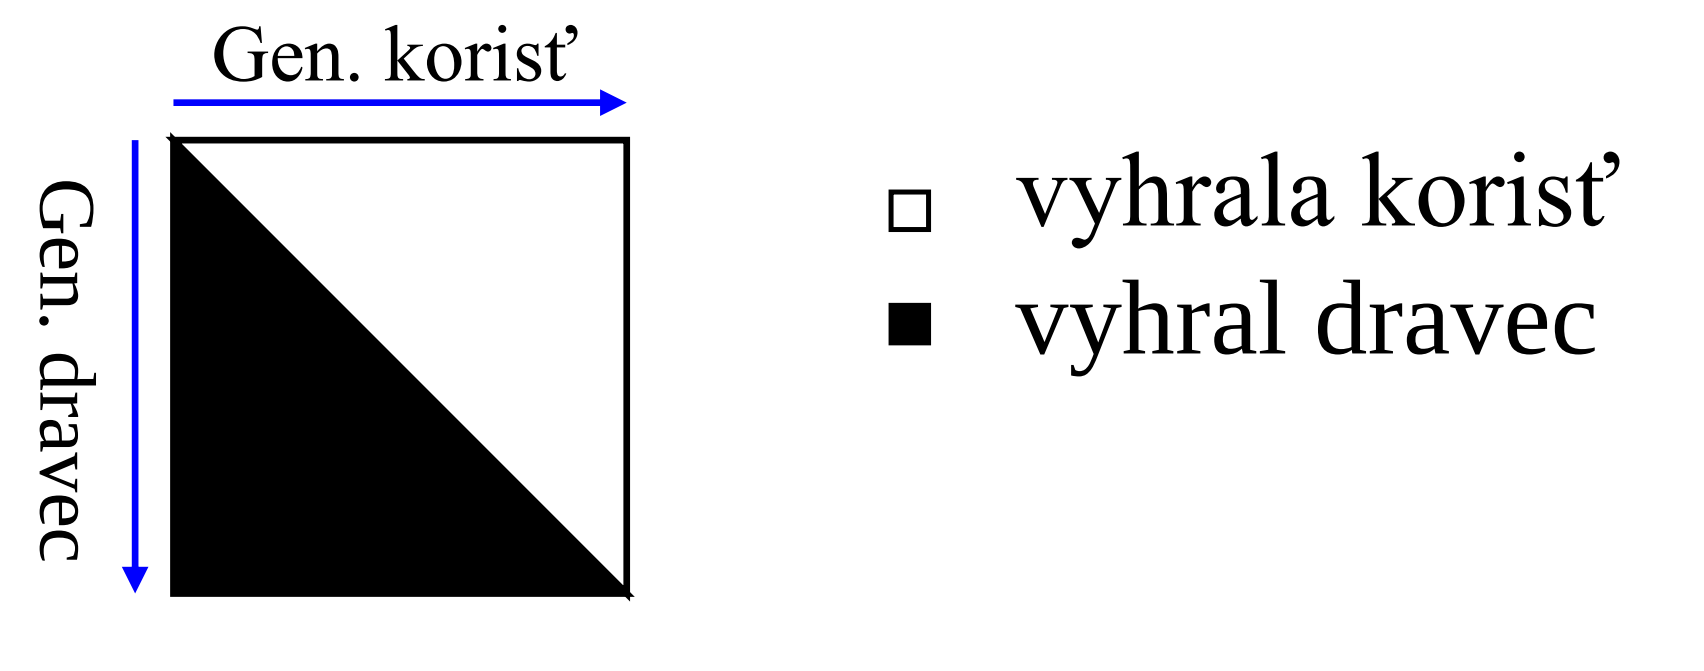
\includegraphics[width=0.4\textwidth]{img/ciao.png}
\caption{CIAO obrázek ukazující \uv{ideální} výsledek (nejlepší z nové generace vždy porazí nejlepší z předchozích)}
\end{figure}

\item[Mistrovství] Vyhodnocení \textit{po skončení evoluce}. Necháme soupeřit nejlepšího z každé generace s nejlepšími soupeři \textit{ze všech} generací(tj. nejen z předchozích. \uv{Fitness} jedince je pak množství vítězství.
\end{description}

\begin{figure}[H]
\centering
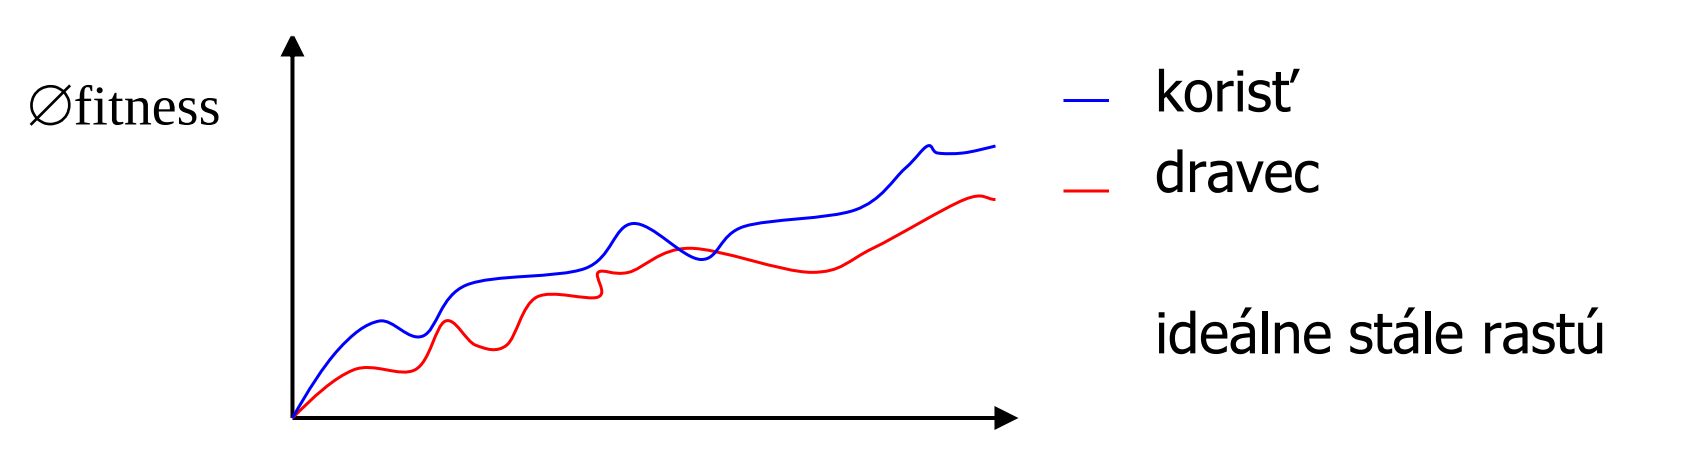
\includegraphics[width=0.7\textwidth]{img/mistrovstvi.png}
\end{figure}


\subsubsection{Zacyklení strategií}
Typickým problémem kompetitivní koevoluce je \textbf{zacyklení} strategií. Tj. existuje množina efektivních chování jako reakce na chování soupeře, jakmile však změním strategii, změní ji i soupeř, na což reaguji svou změnou strategie, \dots Toto chování by ideálně mělo najít optimální strategii pro všechny strategie soupeře, často se ale stává, že se zacyklíme. 

Příklad pro roboty dravec-kořist:
\begin{itemize}
\item\textbf{Strategie dravce}
	\begin{itemize}
	\item D1: pronásleduj kořist
	\item D2: \uv{číhej}, tj. zůstaň na místě, sleduj kořist a zaútoč pouze pokud se kořist přiblíží
	\end{itemize}
\item\textbf{Strategie kořisti}
	\begin{itemize}
	\item K1: stůj na místě (u stěny)
	\item K2: rychle se pohybuj a vyhýbej se dravci (i stěnám)
	\end{itemize}
\end{itemize}
Na každou strategii dravce funguje nějaká strategie kořisti a naopak: D1 $>$ K1 $>$ D2 $>$ K2 $>$ D1 $>$ \dots



%TODO koevoluce
TODO koevoluce


\subsection{Otevřená evoluce}
Evoluce bez konce, tj. neexistuje ukončovací podmínka ani optimální řešení, neboť fitness funkce je \textit{dynamická}. Často je dynamické i kódování jedince -- např. pokud u neuroevoluce mohou síti ubývat a přibývat neurony či synapse. 

Míra změn fitness může být různá: 
\begin{description}
	\leftskip 30pt
	
	\item[malé změny] robot se opotřebuje, v chemické továrně se trochu změní suroviny apod.
	\item[výrazné morfologické změny] vrcholy zanikají, nové vznikají, \uv{emerging markets}
	\item[cyklické změny] roční období, spotřeba elektřiny, \dots
	\item[katastrofické změny] bouchla elektrárna, nehoda na dálnici, \dots
\end{description}

Byly navrženy různé postupy pro vyrovnání se s dynamickou fitness. Například \textit{vyvolaná hypermutace} (při snížení fitness), \textit{náhodná migrace} (při snížení fitness se generují noví náhodní jedinci) a obecně metody vedoucí k udržení diverzity populace: zmenšení selekčního tlaku, crowding, niching, subpopulace, dynamické druhy (které se množí jen mezi sebou).

Dynamická fitness je vyvolaná i kompetitivní koevolucí, a tedy evoluční souboje typ lovec-kořist lze označit za otevřenou evoluci.


%TODO otevřená evoluce


\section{Rojové optimalizační algoritmy.}
\subsection{Optimalizace hejnem částic}
Anglicky \textit{particle swarm optimization} -- jedná se o populační prohledávací algoritmus inspirovaný hejny ptáků/hmyzu/ryb. Jedinec se nazývá \textbf{částice} a jde typicky o vektor reálných čísel. Neexistují křížení ani mutace, jak je známe.

\subsubsection{Algorimus}
\begin{minipage}{\linewidth}
	\begin{lstlisting}[frame=single, escapeinside={\%*}{*)}]
init each particle
while not (max iterations or minimum error)
	foreach particle p:
		f = fitness(p)
		if f > p.pBest
			p.pBest = f
	gBest = max(p.pBest for each particle p)			
	foreach particle p:
		p.v = p.v + 
			+ c1 * rand(0,1) * (pBest - p.position) 
			+ c2 * rand(0,1) * (gBest - p.position) 
		p.position += p.v		
	\end{lstlisting}
\end{minipage}

Každá částice má rychlostní vektor $v$, který se aktualizuje podle nejlepší pozice částice v historii (řádek 10) a nejlepší globální pozice v historii (řádek 11). Učicí konstanty c1,c2 se často nastavují na c1 = c2 = 2. \\
\textit{Pozn. celé to asi může být v jednom for cyklu s tím, že gBest se aktualizuje průběžně a ne po "generacích".}

PSO jsou podobné GA -- stochastický model, fitness pro ohodnocení, náhodná iniciální konfigurace atd. -- ale současně se v mnohém liší: neexistují genetické operace, částice mají paměť a výměna informací probíhá pouze od nejlepších částic ostatním. 

PSO nepoužívají gradient pro optimalizaci, což znamená, že optimalizovaná funkce nemusí být diferencovatelná.


\subsection{Další rojové optimalizační algoritmy}
Obecně se definuje \textbf{Swarm Intelligence (SI)} jako \textit{“The emergent collective intelligence of groups of simple agents"}. Dvě základní vlastnosti jsou sebeorganizace a dělba práce. Kromě PSO sem lze zařadit ještě Ant Colony Optimization (ACO), Artificial Bee Colony (ABC), Glowworm Swarm Optimization, Cuckoo Search Algorithms a v jistém směru sem spadá i diferenciální evoluce (jelikož je population-based). Kromě DE se tyto algoritmy (a mnohé další, třeba i simlated annealing)  označují také nálepkou \textit{metaphor-based metaheuristics}, a to díky tomu, že jsou typicky insipirované nějakou reálnou skutečností (chování roje, chování mravenců, zpracování kovů apod.). Tyto se staly terčem kritiky pro nedostatek inovace a efektivity, kterou schovávají právě za poutavou metaforou (\url{https://en.wikipedia.org/wiki/List_of_metaphor-based_metaheuristics}).

\subsubsection{Ant Colony Optimization (ACO)}
Systém inspirovaný chování mravenců při hledání potravy, konkrétně použitím feromonů. V podstatě jde o techniku nalezení nejlepší cesty v grafu. Agent (mravenec) se pohybuje v grafu a zanechává za sebou feromonovou stopu. Pohyb se řídí rovnicí:
$$p^k_{ij}(t) = \frac{([\tau_{ij}(t)]^\alpha \cdot [\eta_{ij}]^\beta)}{(\sum\limits_{n \in J_k}[\tau_{in}(t)]^\alpha \cdot [\eta_{in}]^\beta)}$$

$p^k_{ij}(t)$ je pravděpodobnost přechodu mravence $k$ z uzlu $i$ do uzlu $j$ v čase $t$, $J_k$ jsou uzly, kam má mravenec $k$ povoleno jít, $\eta_{ij}$ symbolizuje \uv{viditelnost} mezi $i$ a $j$ a $\tau_{ij}(t)$ reprezentuje množství nevypařeného feromonu mezi $i$ a $j$ v čase $t$. Parametry $\alpha$ a $\beta$ kontrolují, nakolik prohledávání závisí na feromonech. Každý mravenec $k$ má také tabu list navštívených uzlů, aby nenavštívil nějaký dvakrát.

Umístění feromonů se řídí rovnicí:
\[
\Delta\tau^k_{ij} = 
\begin{cases}
	\frac{Q}{L_k}(t) 	& \quad \text{leží-li hrana $ij$ na cestě mravence $k$} \\
	0 					& \quad \text{jinak}\\
\end{cases}
\]

$Q$ je konstanta, $L_k$ je cena cesty (její délka), $k$ je mravenec, $t$ je čas (iterace).

Feromony se časem vypařují. Celková změna feromonu na hraně $ij$ je tedy:
$$\tau_{ij}(t+1) = (1-p)\tau_{ij}(t) + \sum_{k=1}^m [\Delta\tau^k_{ij}(t)]$$
kde $m$ je počet mravenců a $p$ je míra vypařování. To je důležitý parametr algoritmu, který ovlivňuje poměr mezi explorací a exploatací.

Mírně vylepšená varianta ACO je Ant Colony System (ACS).

Dobrý přehled dalších algoritmů (např Artificial Bee Colony) lze nalézt na \url{http://journals.plos.org/plosone/article?id=10.1371/journal.pone.0122827}






\section{Memetické algoritmy, hill climbing, simulované žíhání.}
\textbf{Memetické algoritmy} jsou EA obohacené o lokální prohledávání uvnitř cyklu. Základní princip je ten, že evolucí vyvinutý jedinec ještě před ohodnocením podstoupí proceduru lokálního prohledávání -- to může být např. hill climbing, simulované žíhání nebo backpropagation u ANN). 

Inspirováno \textbf{mémy} (angl. \textit{meme} (čti /mi:m/)), což jsou ideje/myšlenky šířící se ve společnosti, které mohou podstoupit mutaci či selekci, stejně jedinci v klasické evoluci. 

Alternativně jsou MA označovány jako \textit{Baldwinian EA}, \textit{Lamarckian EA} nebo jako \textit{genetic local search}.

\subsubsection{Algoritmus}
\begin{minipage}{\linewidth}
	\begin{lstlisting}[frame=single, escapeinside={\%*}{*)}]
t = 0, initialize P[0]
P[0].localSearch()
evaluate(P[0])
while notTerminated do
	P[t] = selectIndividuals()
	mutate(P[t])
	P[t].localSearch()
	evaluate(P[t])
	P[t+1] = buildNextGen(P[t])
	t++

	\end{lstlisting}
\end{minipage}

\subsubsection{Existují dva přístupy, co dělat s výsledkem:}
\begin{description}
	
	
	\item[Lamarckismus] Když prohledáváním najdu lepšího jedince, vezmu ho (to je ovšem darwinisticky nekorektní, změnil jsem genotyp na základě fenotypu).
	\item[Baldwinismus] Když lokálním prohledáváním najdu lepšího jedince, vezmu jen jeho fitness (ale neměním genotyp).
\end{description}


\subsubsection{Hill climbing}
Nejjednodušší informovaná metoda lokálního prohledávání stavového prostoru. Vstupem je uzel, ze kterého se má prohledávání zahájit. Nejprve je uzel expandován - jsou vygenerovány jeho sousední uzly a tyto uzly jsou ohodnoceny. Algoritmus vybere z nich nejlépe ohodnocený uzel a ten je nadále expandován. 

Algoritmus tak expanduje uzly se stále vyšším ohodnocením, dokud nenarazí na uzel po jehož expanzi mají všechny jeho sousední uzly horší ohodnocení. Algoritmus nemá paměť, navštívené uzly okamžitě zapomíná.

\medskip\textbf{Varianty:}
\begin{description}
	\leftskip 30pt
	
	\item[first choice HC vs. steepest ascent HC] First choide HC vezme prvního lepšího souseda, steepest zkusí všechny a vezme nejlepšího.
	\item[stochastic HC] Ze zlepšujících sousedů vybere náhodně podle míry zlepšení.
	\item[random restart HC (or shotgun HC)] Náhodné restarty v různých místech, částečně řeší problém uvíznutí v lokálním optimu.
\end{description}


\subsubsection{Simulované žíhání}
	\setlength\intextsep{0pt}
\begin{wrapfigure}{r}{0.35\textwidth}
	\centering

	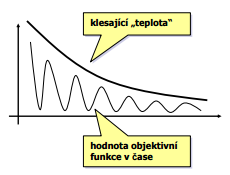
\includegraphics[width=0.3\textwidth]{img/simulated_annealing.png}
\end{wrapfigure}
Lokální prohledávání kombinující HC a náhodnou procházku. Algoritmus náhodně volí stav okolí a vydá se do něj pokud:
\begin{itemize}
	
	
	\item je lepší než aktuální stav
	\item je horší, ale zhoršení je povoleno s určitou mírou pravděpodobnosti odvozenou od aktuální \textbf{teploty}; teplota se přitom postupně snižuje podle „ochlazovacího“ schématu
\end{itemize}


\subsubsection{Algoritmus}
\begin{minipage}{\linewidth}
\begin{lstlisting}[frame=single, escapeinside={\%*}{*)}]
	current = init()
	for t = 1 to %*$\infty$*)
		T = schedule(t)
		if T = 0 then 
			return current
		next = randomNeighbor(current)
		%*$\Delta$E*) = f(next) - f(current)
		if (%*$\Delta$E*) > 0) or (%*$e^{\Delta{}E/T} < $*) rand(0,1))
			current = next
\end{lstlisting}
\end{minipage}






\section{Aplikace evolučních algoritmů (evoluce expertních systému, neuroevoluce, řešení kombinatorických úloh, vícekriteriální optimalizace).}
\subsection{Evoluce expertních systémů}
Expertní systémy jsou modely z oblasti \textit{strojového učení}, jejichž základní charakteristikou je, že pro výpočet svého výstupu používají pravidla IF: THEN. Zastupují tedy větev strojového učení založenou na \textit{formální logice} (druhá, protikladná větev, reprezentovaná především neuronovými sítěmi, je založena na \textit{konekcionismu}, tj. modeluje biologické fungování mozku, nikoli logické). Expertní systémy, které se učí pomocí simulované evoluce, se nazývají \textbf{learning classifier systems (LCS)}. Existují dvě základní paradigmata: \textit{michiganský přístup} (jedinec je pravidlo) a \textit{pittsburghský přístup} (jedinec je množina pravidel).

\begin{wrapfigure}{r}{0.45\textwidth}
\centering
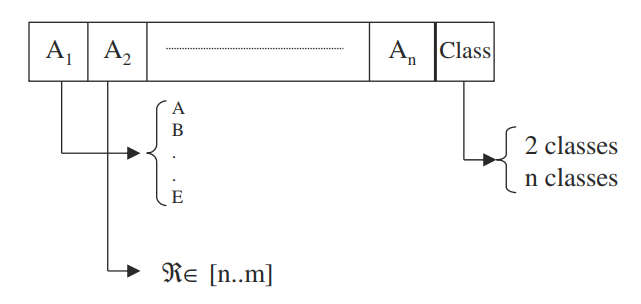
\includegraphics[width=0.4\textwidth]{img/classification_instance.png}
\end{wrapfigure}
Nejprve ještě ke klasifikaci obecně. \textbf{Klasifikační úloha} spočívá v označování předkládaných instancí z nějaké domény správnou \uv{nálepkou}, jejich přiřazení do nějaké \textbf{třídy} (kterých je omezená množina, často pouze dvouprvková). \textbf{Instance} mají pevnou strukturu danou konkrétní problémovou doménou, která se dá vyjádřit pevným počtem \textbf{atributů} (nebo \textit{příznaků, angl. features}), které charakterizují tuto instanci; a v případě anotovaného datasetu má instance jako atribut i správnou třídu. Atributy obecně mohou být nominální (prvek nějaké konečné množiny), diskrétní nebo spojité.


\subsubsection{Pittsburghský přístup}
Pittsburghský přístup je nejbližší klasickému GA. Jedinec v populaci je kompletní množina pravidel řešící daný problém. Tato množina může být různě velká, máme tedy jedince variabilní délky. Při klasifikaci může dojít ke \textit{konfliktu pravidel}, tj. více pravidel může být použito pro klasifikaci dané instance -- to lze řešit např. utříděním pravidel do seznamu, pak se z pravidel \uv{matchujících} danou instanci aplikuje to s nejnižším pořadovým číslem. \textbf{Genetické operátory} jsou poměrně komplikované, typicky jich je více a některé fungují na úrovni celých množin, některé na úrovni jednotlivých pravidel a některé na úrovni termů v pravidlech. 

\textbf{Fitness} jedince se počítá takto: pro každou instanci v trénovací množině se vezme první matchující pravidlo a přiřadí se třída daná tímto pravidlem -- ta se porovná s očekávanou třídou (trénovací vzorky jsou anotované). Fitness je pak dána procentem úspěšně klasifikovaných instancí.

Konkrétním reprezentantem pittsburghského přístupu je například systém GABIL. Ten je určen pro řešení \textit{binární} klasifikace (tj. pouze 3 třídy) a funguje pouze pro domény s \textit{nominálními} atributy. Jednotlivá pravidla (tzv. \textit{komplexy}) jsou ve formátu \textit{predikát $\rightarrow$ třída}, kde predikát je výraz v konjunktivně normální formě (CNF) ve tvaru
$$(A_1 = V_1^1 \lor \dots \lor A_1 = V_1^m) \land \dots \land (A_n = V_n^1 \lor \dots \lor A_n = V_n^m)$$
kde $A_i$ je $i$-tý atribut a $V_i^j$ je $j$-tá hodnota $i$-tého atributu. Taková pravidla lze pak zapsat pomocí binárního řetězce, například 
$$1100|0010|1001|1$$
tedy vyjadřuje pravidlo: pokud první atribut nabývá první či druhé hodnoty, druhý atribut třetí hodnoty a třetí atribut první nebo čtvrté hodnoty, pak instance patří do třídy 1. 

Na těchto binárních řetězcích lze pak snadno aplikovat genetické operátory. Ty fungují na různých úrovních:
\begin{description}
	
	
	\item[na úrovni jedince (množiny pravidel)] výměna pravidel, kopírování pravidel, generalizace pravidla, smazání pravidla, specializace pravidla, zahrnutí jednoho pozitivního příkladu
	\item[na úrovni komplexů] rozdělení komplexu na 1 selektoru, generalizace selektoru (nahrazení 11\dots1), specializace
	generalizovaného selektoru, zahrnutí negativního příkladu
	\item[na selektorech] mutace $0 \leftrightarrow 1$, rozšíření $0 \rightarrow 1$, zúžení $1 \rightarrow 0$,
\end{description}

\subsubsection{Michiganský přístup}
Zde je jedincem v populaci pravidlo. V klasickém GA typicky dojde ke konvergenci populace k jedinému řešení -- my ale chceme získat množinu pravidel, ideálně docela ortogonálních. Jednou možností je \textbf{Iterative Rule Learning} přístup, který postupně generuje pravidla iterativním spouštěním GA. Tj. spustí se GA, najde se nejlepší pravidlo, to se uloží a z trénovací množiny se odstraní všechny správně klasifikované instance. Toto se opakuje, dokud není trénovací množina prázdná.

Michiganský přístup funguje trochu jinak. Na klasifikaci se podílí \textit{celá populace}. Evoluce neprobíhá po generacích, nýbrž jen občas a jen na části populace. Konkrétně lze rozlišit fázi \textit{objevování nových pravidel} (pomocí GA) a fázi \textit{učení}, během které dochází k odměňování/penalizaci jedinců, jak si vedou při klasifikaci -- od toho je pak odvozena jejich fitness.

Pravidla mohla mít na pravé straně kromě klasifikačního výstupu i další příznaky, tzv \uv{zprávy}. Na levé straně pravidel se pak mohly vyskytovat \uv{receptory} pro jejich příjem. Celý systém má frontu zpráv.

Problémem při klasifikaci celou populací realizace algoritmu odměn pro pravidla. Původní Hollandův návrh obsahoval tzv. \textit{bucket brigade}: pravidla musejí dát část svého \uv{kreditu}, když chtějí soupeřit o možnost být v cestě k řešení. Tento systém byl ale poměrně těžkopádný. 

Zjednodušením tohoto systému byl \textbf{ZCS (Zero Classifier System)}. Neměl vnitřní zprávy ani žádný složitý systém alokace odměn. Síla pravidel se upravovala podle jednoduchého algoritmu:
\begin{itemize}
	
	
	\item pravidlům, která odpovídají vstupu, ale mají jiný výstup, se síla zmenší násobením konstantou $0 < T < 1$
	\item všem pravidlům se zmenší síla o malou část B
	\item tahle síla se rozdělí rovnoměrně mezi pravidla, která \textit{minule} odpověděla správně, zmenšená o faktor $0<G<1$
	\item nakonec, odpověď od systému se zmenší o B a rozdělí rovnoměrně mezi pravidla, která \textit{teď} odpověděla správně
\end{itemize}
Inovací bylo přidání \textbf{cover} operátoru. Ten řešil případy, kdy nebylo žádné pravidlo pro daný vstup. Pak bylo vygenerováno ad hoc. Pravidla jsou ve formátu $01\#|0$, kde 1 znamená \uv{příznak nastal}, 0 opak a $\#$ je \uv{žolík}. Pro nebinární nominální atributy lze samozřejmě použít rozšířenou abecedu. Ad hoc pravidlo bylo tedy vygenerováno tak, že se nějaké náhodné vstupní atributy nahradily $\#$ a zvolil se náhodný výstup.

Dalším vylepšením byl systém \textbf{XCS}, který zakládá fitness pravidla na jeho přesnosti, nikoliv \uv{výdělku}, tj. dává šanci prosadit se i pravidlům, která vedou k akcím s malou odměnou. Tímto je podpořeno vyvíjení komplexního systému pravidel pokrývajícího co nejvíce případů.




\subsection{Neuroevoluce}
\label{neuroevolution}
Neuronové sítě se klasicky učí pomocí nějaké varianty backpropagation, ale jsou situace, kdy může být lepší pokusit se vyvinout optimální síť (řešící daný problém) pomocí EA. Mnohdy nelze \textit{učení s učitelem} použít vůbec -- například v robotice -- a je nutno spoléhat na \textit{zpětnovazební učení} (reinforced learning).

Předmětem evoluce mohou být synaptické váhy, struktura sítě, nebo obojí najednou. 

Existují i hybridní přístupy, kdy jsou EA zkombinovány s lokálním prohledáváním. Je například možno pomocí GA najít počáteční vah a poté síť doučit pomocí klasické BP $\rightarrow$ výsledná fitness (BP je citlivé na počáteční nastavení vah).

\subsubsection{Učení vah}
Nejjednodušší je zakódovat váhy do vektoru a pak použít klasický floating point GA se standardními genetickými operátory. Problémy: mnoho parametrů optimalizováno naráz (stovky až tisíce hodnot synaptických vah); různé vzájemně si konkurující kódy reprezentují funkčně totožné sítě; předčasná konvergence. (Jednoduché) křížení navíc nefunguje příliš dobře, neboť výsledné vektory často nekódují validní síť.

\subsubsection{Učení struktury}
Prostor možných architektur je nekonečný a především nediferencovatelný, takže gradientní metody jsou k ničemu. Evoluce však může fungovat bez problémů.
Strukturu sítě lze zakódovat několika způsoby:
\begin{description}
	
	
	\item[přímé kódování] -- binární matice synapsí, před evolucí se typicky převedou na jeden dlouhý linearizovaný vektor 
	\item[gramatické kódování] 2D formální gramatiky, které jsou \uv{programem} pro vytvoření matice	
	\item[růst sítě ve 2D] rané pokusy v evoluční robotice, velmi neefektivní
	\item[celulární kódování] v podstatě Genetické programování -- program obsahuje instrukce, jak zkonstruovat síť (operace typu: přidej neuron, rozděl neuron sériově/paralelně, přepoj synapsi apod.)
\end{description}

\subsubsection{Evoluce částečných sítí}
\setlength\intextsep{0pt}
\begin{wrapfigure}{r}{0.5\textwidth}
	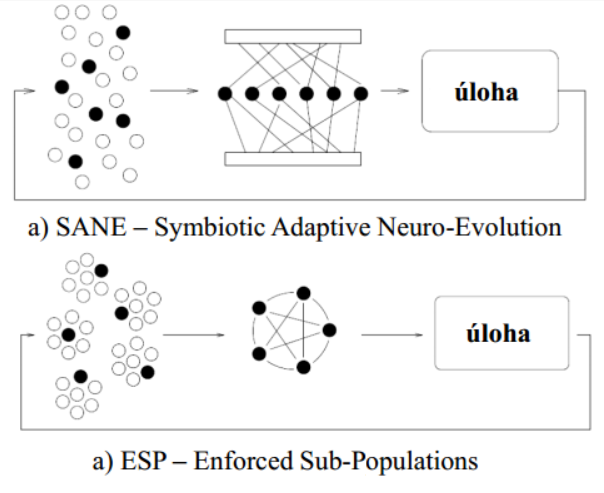
\includegraphics[width=0.5\textwidth]{img/sane_esp.png}
\end{wrapfigure}
\textbf{SANE} (Symbiotic Adaptive Neuroevolution) je variantou neuroevoluce, kdy je struktura pevně daná: jediná skrytá vrstva, pevný počet skrytých neuronů. Jedinci v evoluci jsou neurony (včetně vstupních a výstupních vah). Při ohodnocování se náhodně vybere pevný počet neuronů z populace, postaví se síť a ta se vyhodnotí. Toto se opakuje tak, aby každý neuron z populace byl vybrán aspoň $10\times$. Fitness neuronu je pak průměrná fitness všech sítí, jichž byl součástí.

\textbf{ESP} (Enforced Sub-Populations) funguje na podobném principu, tj. architektura je opět předem daná s pevně daným počtem neuronů (na rozdíl od SANE může být i rekurentní). Rozdíl je v tom, že pro každý z těchto \uv{slotů} se vyvíjejí neurony zvlášť, v oddělených subpopulacích. Takto navržená evoluce podporuje diverzitu (dobrá síť potřebuje různé druhy neuronů), potlačuje redundanci (neurony se vyvíjí pro kompatibilní role) a implicitně rozděluje prohledávaný prostor na podúlohy.


\subsubsection{NEAT (Neuroevolution of Augmenting Topologies)}
Základními charakteristikami algoritmu NEAT jsou: 
\begin{enumerate}
	
	
	\item evoluce topologie společně s vahami
	\item smysluplné křížení pomocí historických značek
	\item ochrana inovací pomocí druhů
\end{enumerate}
Evoluce topologie zahrnuje přidání/odebrání synapse, přidání/odebrání vrcholu. Typicky se začíná od menší sítě, která postupně roste.

Každý neuron a každý synaptický spoj dostanou při svém vzniku svou \textit{historickou značku} (nebo \uv{rodné číslo}). Tato značka se dědí, takže i u různých potomků lze poznat, zda neurony/spoje mají stejný evoluční původ. Při křížení dvou jedinců se potom postupuje takto: pokud se uzel (neuron či spoj) vyskytuje pouze v jednom rodiči, je automaticky zkopírován; pokud se vyskytuje v obou, je náhodně vybrán jeden z nich.
\begin{figure}[H]
	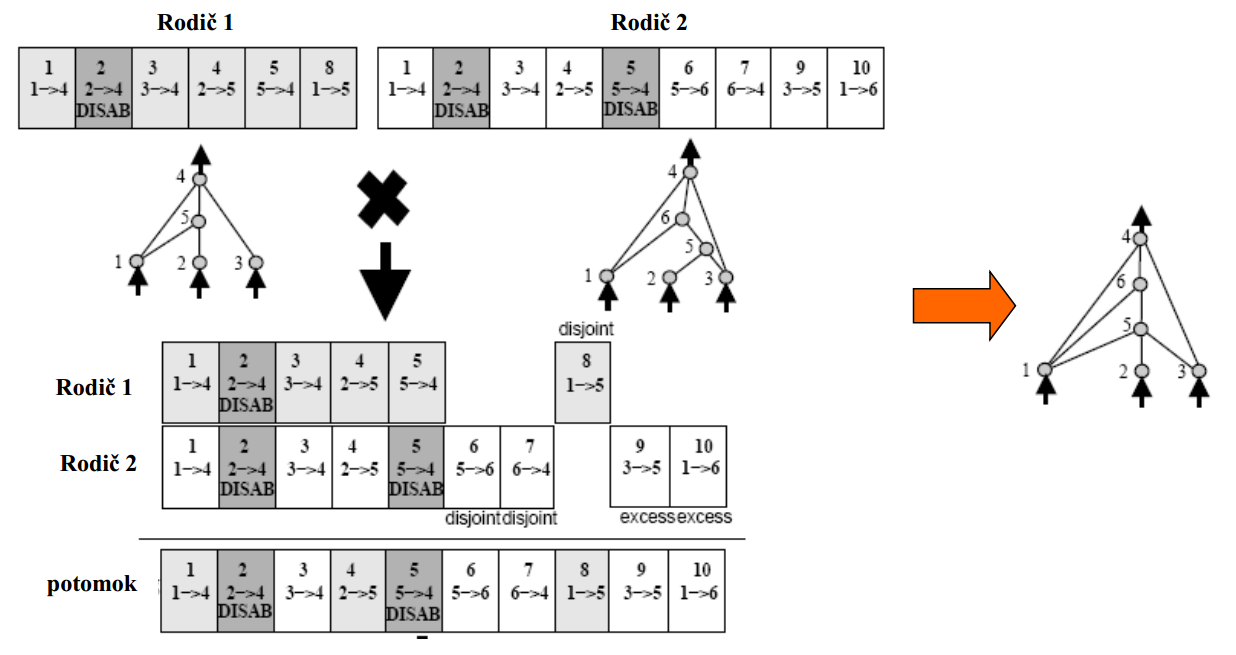
\includegraphics[width=\textwidth]{img/neat.png}
\end{figure}

Když během evoluce vznikne jedinec, který se výrazně liší od ostatních (na to musí být definovaná nějaká metrika), založí se nový \textbf{druh}. Ten je několik generací chráněný -- jedinci nového druhu soutěží pouze mezi sebou.

\subsubsection{HyperNEAT (Hyper-cube NEAT)}
Varianta NEAT, kdy nevyvíjíme síť samotnou, ale jinou síť, která nám naši síť postaví. Tato pomocná síť se nazývá CPPN (Compositional Pattern Producing Network) a liší se od klasických sítí především tím, že v neuronech se místo sigmoidy používají nejrůznější geometrické funkce, např. absolutní hodnota, bipolární sigmoida, Gaussovská funkce, lineární funkce, sinusoida nebo kroková funkce. Na vstupu CPPN je dvojice souřadnic dvou neuronů (pro 2D síť tedy 4 souřadnice: $x_1, y_1, x_2, y_2$), na výstupu je váha, která se má přidělit synapsi mezi neurony na těchto souřadnicích.

Pomocí CPPN tedy můžeme doplnit vhodné váhy do ANN sítě nazývané \textit{substrát}, ta se poté použije pro řešení daného problému. Tato konstrukce umožňuje využít geometrické pravidelnosti daného problému. Příklady použití: šachy, dáma, dravec-kořist, Go, atd. Neurony jsou uspořádány v prostoru daném doménou problému, lze je adresovat souřadnicemi, které využívá CPPN. Síť může být i 3D, kde jednotlivé vrstvy sítě jsou umístěné v různých $z$ souřadnicích.

\begin{figure}[h]
	\centering
	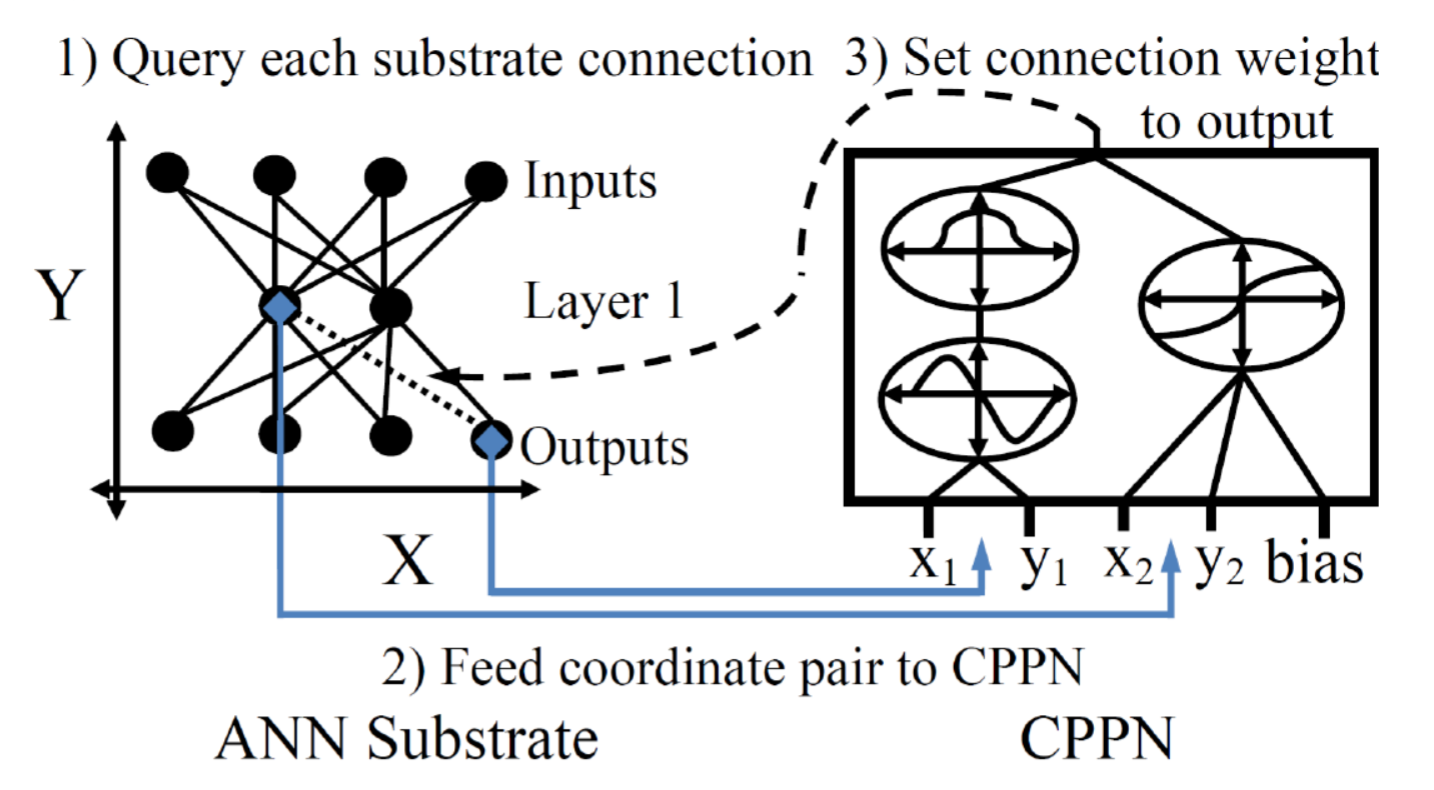
\includegraphics[]{img/hyperneat.png}
\end{figure}

Pro evoluci CPPN se používá klasický NEAT s 2 odlišnostmi: nově vygenerovaný neuron dostane náhodně jednu z geometrických funkcí (namísto sigmoidy); a fitness CPPN se spočte podle správnosti výstupu ANN substrátu vygenerovaného pomocí CPPN.

Substrát lze libovolně škálovat. Můžeme třeba použít dvojnásobný počet neuronů, kterým pak ale přidělíme souřadnice ze stejného intervalu, jako u menšího substrátu.

Zdroj: \url{http://kocmi.tk/photos/DiplomaThesis.pdf}

\subsection{Řešení kombinatorických úloh}
EA jsou velmi vhodné pro řešení NP-těžkých úloh. Rozebereme několik příkladů:

\subsubsection{Batoh (0-1 knapsack problem)}
\textit{Problém:} máme batoh o kapacitě $CMAX$, množinu $n$ věcí, z nichž každá má cenu $v(i)$ a objem $c(i)$. Úkolem je naplnit batoh tak, abychom maximalizovali sumu cen obsažených věcí a současně nepřekročili kapacitu batohu.

\textbf{Kódování:} Binární jedinci délky $n$, přímočará bitová mapa. Např. 0110010 znamená, že bereme věci s indexy 2,3 a 6. Pozor, jedinci nemusí splňovat podmínku o $CMAX$.

\textbf{Operátory:} Lze použít přímočaré křížení, mutaci a klasickou selekci.

\textbf{Fitness:} Bude mít 2 členy: 
$$\max\limits_{B \subset \{1..n\}} \sum\limits_{i \in B} v(i) \text{\ \ a současně\ \ } \min\limits_{B \subset \{1..n\}} CMAX - \sum\limits_{i \in B} c(i)$$

Problém s víceúčelovou optimalizací lze řešit různě:
\begin{itemize}
	
	
	\item Oba členy fitness zvážit a sečíst
	\item Použít jeden z obecných EA pro víceúčelové funkce
	\item Anebo chytře změnit zakódování:
	\begin{itemize}	
		
		
		\item 1 znamená: DEJ věc do batohu POKUD se nepřeplní
		\item takto dosáhneme i toho, že všechny řetězce jsou přípustná řešení
	\end{itemize}
\end{itemize}

\subsubsection{Problém obchodního cestujícího (TSP -- travelling salesman problem)}
\textit{Problém:} Máme $n$ měst, mezi nimi existují cesty definované délky (úplný graf, ohodnocené hrany). Cílem je navštívit všechna města s co nejmenšími náklady -- tj. najít co nejkratší hamiltonovskou kružnici.

\textbf{Fitness:} Délka cesty.

Existuje několik možných reprezentací a na nich závislých genetických operátorů:
\begin{description}
	
	
	\item[reprezentace sousednosti:] Cesta je seznam měst, město $j$ je na pozici $i$, vede-li cesta z $i$ do $j$. Např. (248397156) odpovídá cestě 1-2-4-3-8-5-9-6-7. Některé seznamy negenerují přípustnou cestu. Klasické křížení nefunguje. Schémata fungují, např (*3*\dots) značí všechny cesty s hranou 2-3.
	\item[reprezentace bufferem] Máme buffer vrcholů, třeba uspořádaný. Reprezentace představuje pořadí města v bufferu, města se z bufferu postupně mažou. Např. buffer (123456789) a reprezentace (112141311) kóduje cestu 1-2-4-3-8-5-9-6-7. V této reprezentaci lze použít jednobodové křížení.
	\item[reprezentace permutací] Nejvíce přímočaré: řetězec (517894623) kóduje cestu 5-1-7-8-9-4-6-2-3. Klasické křížení nefunguje, byly navrženy speciální operátory (dobrý přehled viz \footnote{http://www.rubicite.com/Tutorials/GeneticAlgorithms/CrossoverOperators/PMXCrossoverOperator.aspx}):
	\begin{description}
		\leftskip 30pt
		
		\item[PMX (partially mapped crossover] Náhodně vybereme podřetězec z rodiče 1, ten zkopírujeme do nového jedince. Pak se podíváme na tytéž pozice v rodiči 2. Pro každou hodnotu, která se ještě nevyskytuje v budovaném potomkovi, budeme hledat vhodné umístění: nechť chceme umístit hodnotu $h$, která se nachází v rodiči 2 na pozici $i$. Vezmeme hodnotu $h_2$ na téže pozici $i$, ale v rodiči 1. Pak se podíváme, kde se $h_2$ nachází v rodiči 2 -- označme tuto pozici jako $i_2$. Je-li to mimo zkopírovanou oblast, pak jsme našli vhodné umístění a zkopírujeme původní hodnotu $h$ do nového potomka na $i_2$. Je-li $i_2$ uvnitř kopírovaného intervalu, pak pokračujeme v hledání -- do $h_2$ dosadíme hodnotu na $i_2$ v rodiči 1. Viz obr. \ref{pmx}.
		\begin{figure}[H]
			\centering			
			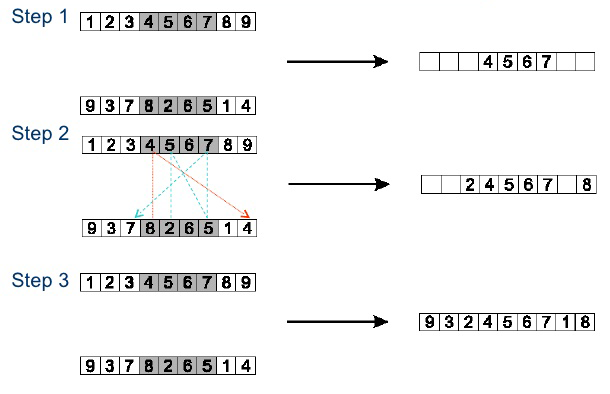
\includegraphics[width=0.6\textwidth]{img/pmx.png}
			\caption{Partially mapped crossover (PMX)}
			\label{pmx}
			
		\end{figure}
		\item[OX (order crossover)] Nejrychlejší křížení. Stejně jako v PMX nejprve vezmeme náhodný podinterval rodiče 1 a beze změny jej zkopírujeme do potomka. Poté vezmeme nepoužité hodnoty z rodiče 2 a počínaje pravým koncem zkopírovaného intervalu je dokopírujeme do potomka.
		
		\begin{figure}[H]
			\centering			
			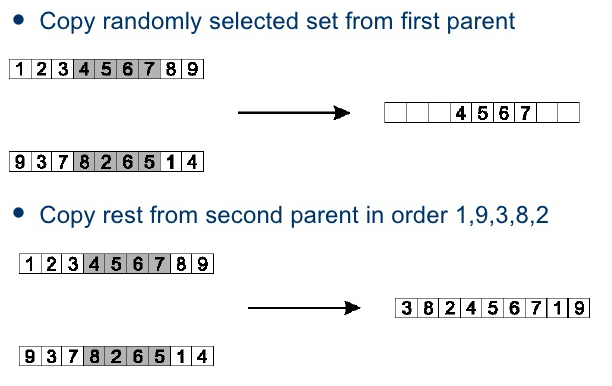
\includegraphics[width=0.6\textwidth]{img/ox.png}
			\caption{Order crossover (OX)}
			\label{pmx}
			
		\end{figure}
		\item[CX (cyclic crossover)] Nejprve jsou identifikovány \uv{cykly} mezi dvěma rodiči: začneme první hodnotou v prvním rodiči, podíváme se na hodnotu na tomtéž indexu v rodiči 2, tuto hodnotu najdeme v rodiči 1, podíváme se na hodnotu na témže indexu v rodiči 2 atd. dokud neuzavřeme cyklus. Takto najdeme všechny cykly. Nového jedince pak vytvoříme kopírováním hodnot po cyklech: hodnoty z prvního cyklu zkopírujeme z prvního rodiče, hodnoty z druhého cyklu z druhého rodiče, hodnoty z třetího cyklu opět z prvního rodiče atd.
		
		\begin{figure}[H]
			\centering			
			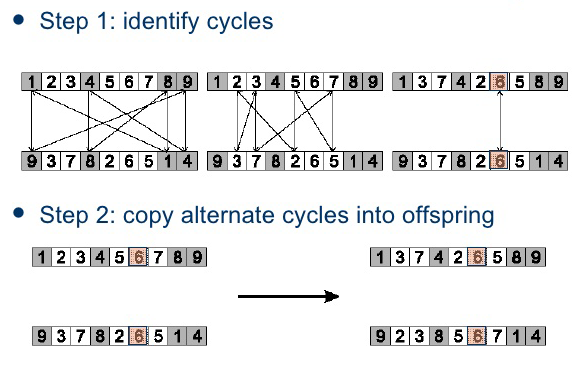
\includegraphics[width=0.6\textwidth]{img/cx.png}
			\caption{Cyclic crossover (CX)}
			\label{cx}
			
		\end{figure}
		
		\item[ER (edge recombination)] Pro každé město si udělám seznam hran, které do/z něj vedou a jsou použity v některém z rodičů. Pak začnu náhodným městem a postupně napojuji další, přičemž vždy ze sousedů vybírám město s nejméně hranami (v případě shody náhodně). Může se stát, že nelze hranu vybrat, ale to se v praxi stává zřídka.
		\item[ER2] Vylepšení: označím si hrany, které jsou dvakrát (tj. v obou rodičích) a při výběru jim dávám přednost. To zachovává ještě více hran z obou rodičů.
		\begin{figure}[H]
			\centering			
			\smallskip
			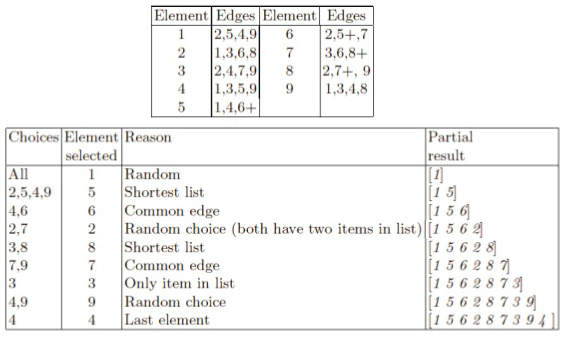
\includegraphics[width=0.6\textwidth]{img/er.png}
			\caption{Edge recombination 2 (ER2): příklad pro rodiče (123456789) a (937826514)}
			\label{pmx}
			
		\end{figure}
		
	\end{description}
\end{description}



Mutace jsou obecně jednodušší (pro všechny reprezentace), používá se:
\begin{itemize}
	
	
	\item inverze podcesty
	\item posun podcesty
	\item záměna 2 měst
	\item záměna podcest
	\item složitější heuristiky: např. \textbf{2-OPT}. Tento \uv{chytrý operátor} funguje tak, že se vyberou dvě hrany, ty se odeberou a nahradí jinými dvěma hranami (je jen jedna možnost). Nakonec se vybere kratší z obou vzniklých cest. Vlastně se jedná o mutaci, která vezme část cesty a tu vloží do jedince v opačném pořadí. 2-OPT se navíc ještě podívá, jestli je výsledek kratší a přijme ho jen pokud je.
	
	2-OPT se přirozeně dá zobecnit na \textbf{$k$-OPT}, odstraní se $k$ hran a vzniklé fragmenty se pospojují tak, aby výsledná cesta byla co možná nejkratší.
\end{itemize}

Úspěšnost evoluce závisí také na inicializaci. Nejpoužívanější jsou dvě varianty:
\begin{description}
	
	
	\item[nejbližší sousedi] Začni s náhodným městem, postupně vybírej jako další to nejbližší z dosud nevybraných.
	\item[vkládání hran] Budujeme cestu T, na začátku náhodná hrana. K cestě T vyber nejbližší město c mimo T. Najdi hranu k-j v T tak, že minimalizuje rozdíl mezi k-c-j a k-j. Vyhoď k-j, vlož k-c-j do T.
\end{description}

\subsection{Vícekriteriální optimalizace (MOEA -- Multi-objective EA)}
Velmi často potřebujeme optimalizovat více funkcí současně, tj. místo jedné fitness jich máme celý vektor $\overline{f} = (f_1, f_2, \dots f_n)$. Ty si často odporují, nelze tedy najít řešení optimální pro všechny zároveň.

\begin{wrapfigure}{r}{0.45\textwidth}
	\centering
	
	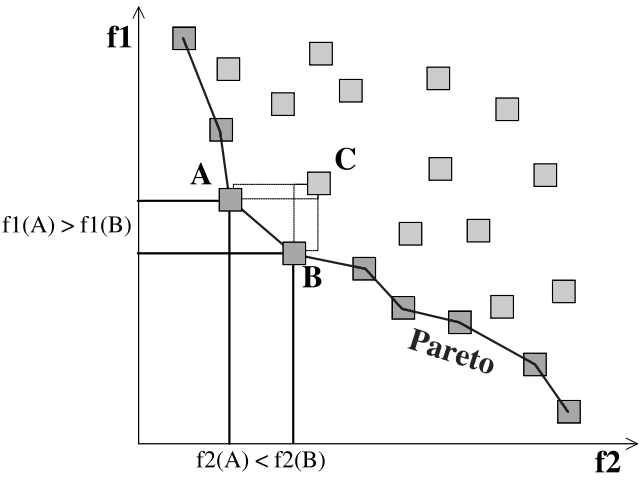
\includegraphics[width=0.4\textwidth]{img/pareto.png}
\end{wrapfigure}

Řekneme, že řešení $x$ \textbf{slabě dominuje} řešení $y$, jestliže $x$ je ve všech kritériích aspoň tak dobré jako $y$, tj. $f_i(x) \leq f_i(y)\quad \forall i \in \{1,\dots,n\}$. 

Řekneme, že $x$ \textbf{dominuje} $y$, když jej slabě dominuje a navíc je aspoň v jedno kritériu lepší, tj. $\exists j: f_j(x) < f_j(y)$. 

Řešení $x$ a $y$ jsou \textbf{nesrovnatelná}, jestliže $x$ nedominuje $y$ a $y$ nedominuje $x$.

\textbf{Pareto-optimální řešení} (Paretova fronta, Pareto-optimální fronta) je množina jedinců, kteří nejsou dominováni žádným jiným jedincem. Je často nekonečná, hledáme konečnou aproximaci.

V případě MOEA není jeden nejlepší jedinec v populaci, používá se celá populace a považuje se za aktuální aproximaci Pareto-optimální množiny řešení. 

\subsubsection{Algoritmy}
Hlavní rozdíl mezi jednokriteriálními a vícekriteriálními algoritmy je v selekci (operátory mohou klidně zůstat stejné). S čímž samozřejmě souvisí způsob, jakým se počítá fitness. Celkově je potřeba zajistit konvergenci k Pareto optimální frontě a zároveň zajistit i dobré pokrytí této fronty.
\begin{description}
	
	
	\item[Agregace fitness] Nejjednodušší přístup. Definujeme agregovanou fitness $f$ jako váženou sumu všech $f_i$ a problém řešíme jako klasickou jednokriteriální optimalizaci. Problémem je nastavení vah u jednotlivých $f_i$.
	\item[VEGA (Vector Evaluated GA)] Populaci $N$ jedinců utřídím podle každé z $n$ fitness funkcí, poté pro každé $i$ vyberu $\frac{N}{n}$ nejlepších jedinců dle $f_i$. Na ty poté aplikuji křížení, mutaci a provedu selekci do další generace. 
	
	Nevýhodou tohoto přístupu je obtížné udržování diverzity populace a často dochází ke konvergenci k extrémům jednotlivých $f_i$.
	\item[NSGA (Non-dominated sorting GA)] Fitness se počítá pomocí dominance, diverzitu populace zaručuje \textbf{niching}.
	
	Populace $P$ je rozdělena na postupně konstruované fronty $F_1$, $F_2$, \dots, a to takto: 
	\begin{itemize}
		
		
		\item $F_1$ je množina všech nedominovaných jedinců z $P$
		\item $F_2$ je množina všech nedominovaných jedinců z $P-F_1$
		\item $F_3$ je množina všech nedominovaných jedinců z $P - (F_1 \cup F_2)$
		\item \dots
	\end{itemize}
	
	Pro každého jedince $i$ ve frontě $F_k$ se spočte jeho \textit{niching faktor} jako
	$$sh(i) = \sum_{j \in F_k} sh(i,j)$$
	kde 
	$$
	sh(i,j) = 
	\begin{cases}
		1 - \left(\frac{d(i,j)}{dshare}\right)^2 	& \quad \text{pro $d(i,j) < dshare$} \\
		0 											& \quad \text{jinak}\\
	\end{cases}
	$$
	kde $d(i,j)$ je vzdálenost $i$ a $j$, $dshare$ je předem daný parametr. Niching faktor tedy vyjadřuje, jak blízko jsou další jedinci v populaci. Čím blíže 0, tím osamocenější jedinec je, naopak hodnota blízká 1 znamená mnoho blízkých sousedů.
	
	Jedinci z $F_1$ dostanou nějakou \uv{dummy fitness} dělenou jejich niching faktorem. Jedinci z $F_2$ dostanou jinou dummy fitness, která je menší než fitness nejhoršího jedince z $F_1$ a opět se dělí jejich niching faktorem; atd.
	
	\item[NSGA II] Odstraňuje nutnost určení $dshare$ -- nahrazuje ji \textbf{crowding distance}, což je součet přes všechna kritéria, vzdálenosti nejbližšího horšího (v daném kritériu) a nejbližšího lepšího jedince. Fitness se pak ve skutečnosti nepočítá, namísto toho se v turnajové selekci porovnávají jedinci nejprve podle čísla fronty (menší je lepší), v případě remízy podle crowding distance (větší je lepší -- jedinci jsou v řídce osídlené oblasti a tedy lépe přispívají k pokrytí fronty).
	
	Dále zavádí elitismus: stará a nová generace jsou spojeny, utříděny a z nich se pak vybírá lepší část do další populace. Postupně se kopírují fronty (od nejlepší) dokud se vejdou do populace, z fronty, která se již nevejde celá, se vybírá podle turnajové metody popsané výše.
	
\end{description}

\subsubsection{Porovnání algoritmů}
Pro porovnání kvality řešení dvou různých algoritmů je třeba vyhodnotit, která z výsledných populací lépe aproximuje Pareto optimální množinu. 
\begin{description}
	
	
	\item[IGD (Inverted Generational Distance)] IGD měří průměrnou vzdálenost každého řeše\-ní na \textit{skutečné} Pareto optimální frontě k nejbližšímu řešení ve výsledné množině. Díky tomu indikátor vyjadřuje jak blízkost řešení k Pareto-optimální frontě (convergence), tak to, jestli jsou řešení po frontě rozmístěna rovnoměrně (spread). Menší hodnoty tohoto indikátoru jsou lepší. 
	\begin{figure}[H]
		\centering
		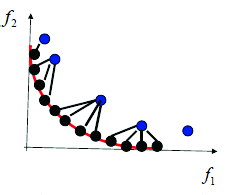
\includegraphics[width=0.4\textwidth]{img/igd.png}
	\end{figure}
	
	\item[Hyperobjem (HV -- hypervolume)] Hyperobjem vyjadřuje objem prostoru dominovaného danou množinou (a omezeného zvoleným referenčním bodem). V případě, že máme jen dvě funkce, které obě najednou minimalizujeme, tak se jedná o plochu \uv{nad} body, které jsou obrazy jedinců v populaci. Plocha je shora omezena referenčním bodem (jinak by byla nekonečná). Tento indikátor opět spojuje jak konvergenci, tak pokrytí Pareto-optimální fronty. Větší hodnoty tohoto indikátoru jsou lepší. Někdy se také jako indikátor používá rozdíl hyperobjemu \textit{skutečné} Pareto optimální fronty a aproximace nalezené algoritmem. Potom jsou samozřejmě lepší menší hodnoty.
	\begin{figure}[H]
		\centering
		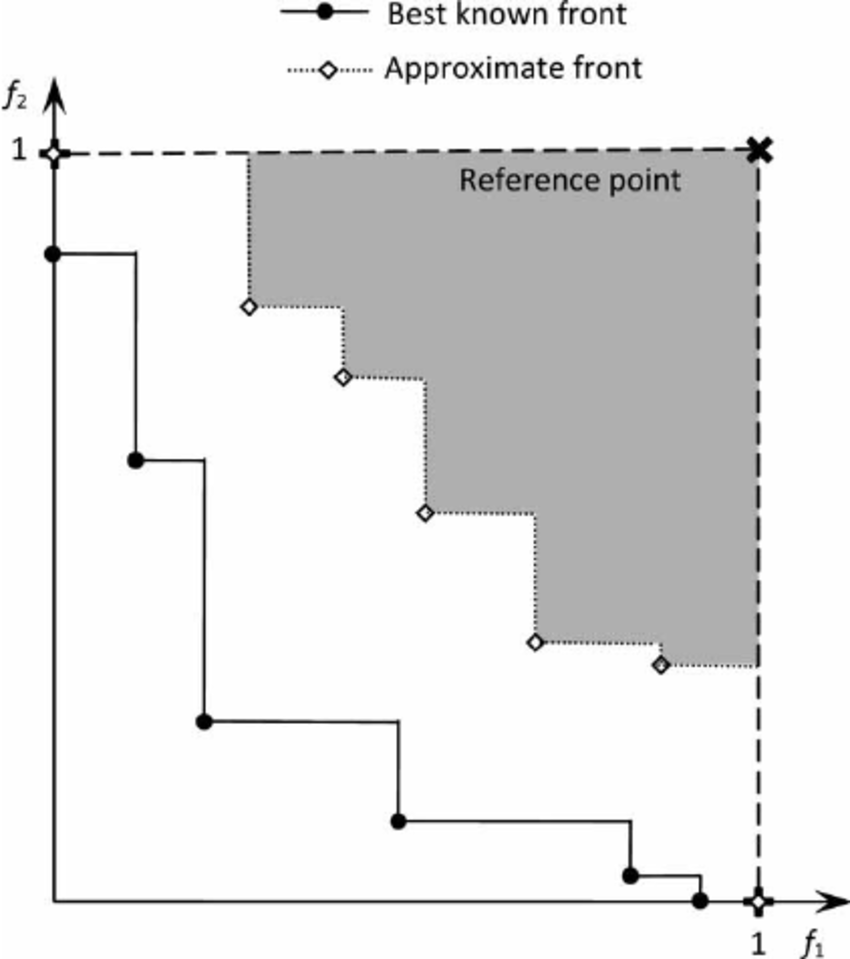
\includegraphics[width=0.35\textwidth]{img/hypervolume.png}
	\end{figure}
	
\end{description}
